\documentclass{ximera}

%% The launch should somehow present a ``mystery'' for the students to
%% solve.  Moreover, it should lead them to the right path. Ideally if we
%% had a bright student working on the launch, they might even develop
%% the techniques from the lesson to solve teh problem. 
%% By the end of the lesson, the mystery is solved!

\title{From average rate of change to instantious rate of change}

\begin{document}
\begin{abstract}
The derivative computes the instantaneous rate of change. 
\end{abstract}
\maketitle

%% Here the idea is to be truthful, enthuastic, and narrow. We want a
%% SINGLE example. So for this prototype we could talk about all kinds
%% of rates of change, but lets refrain from this.


Let me tell you about something that is really awesome: \textit{The
  Global Positioning System.} Seriously, this is a modern ``Wonder of
the World.'' With this system, the secrets of navigating our beautiful
blue sphere are no longer limited to an elite few. Instead we have
devices small enough to fit in our pockets, that cost as little as a
few meals, that can tell us where we are, and even \textit{how fast we
  are going.} Think about this, a mere 2000 years ago, a GPS in the
right hands would have been powerful enough to change the course of
history!

While the details of how GPS works are fascinating, incorporating many
concepts from mathematics and physics, including Einstein's theory of
relativity \ref{see...}, what we are most interested in is how a GPS
computes velocity from position.

The \textit{MOOCulus Team} recently took a road trip from Columbus
Ohio to Urbana-Champaign Illinois in the \textit{MOOCulus Mobile}:
\begin{image}
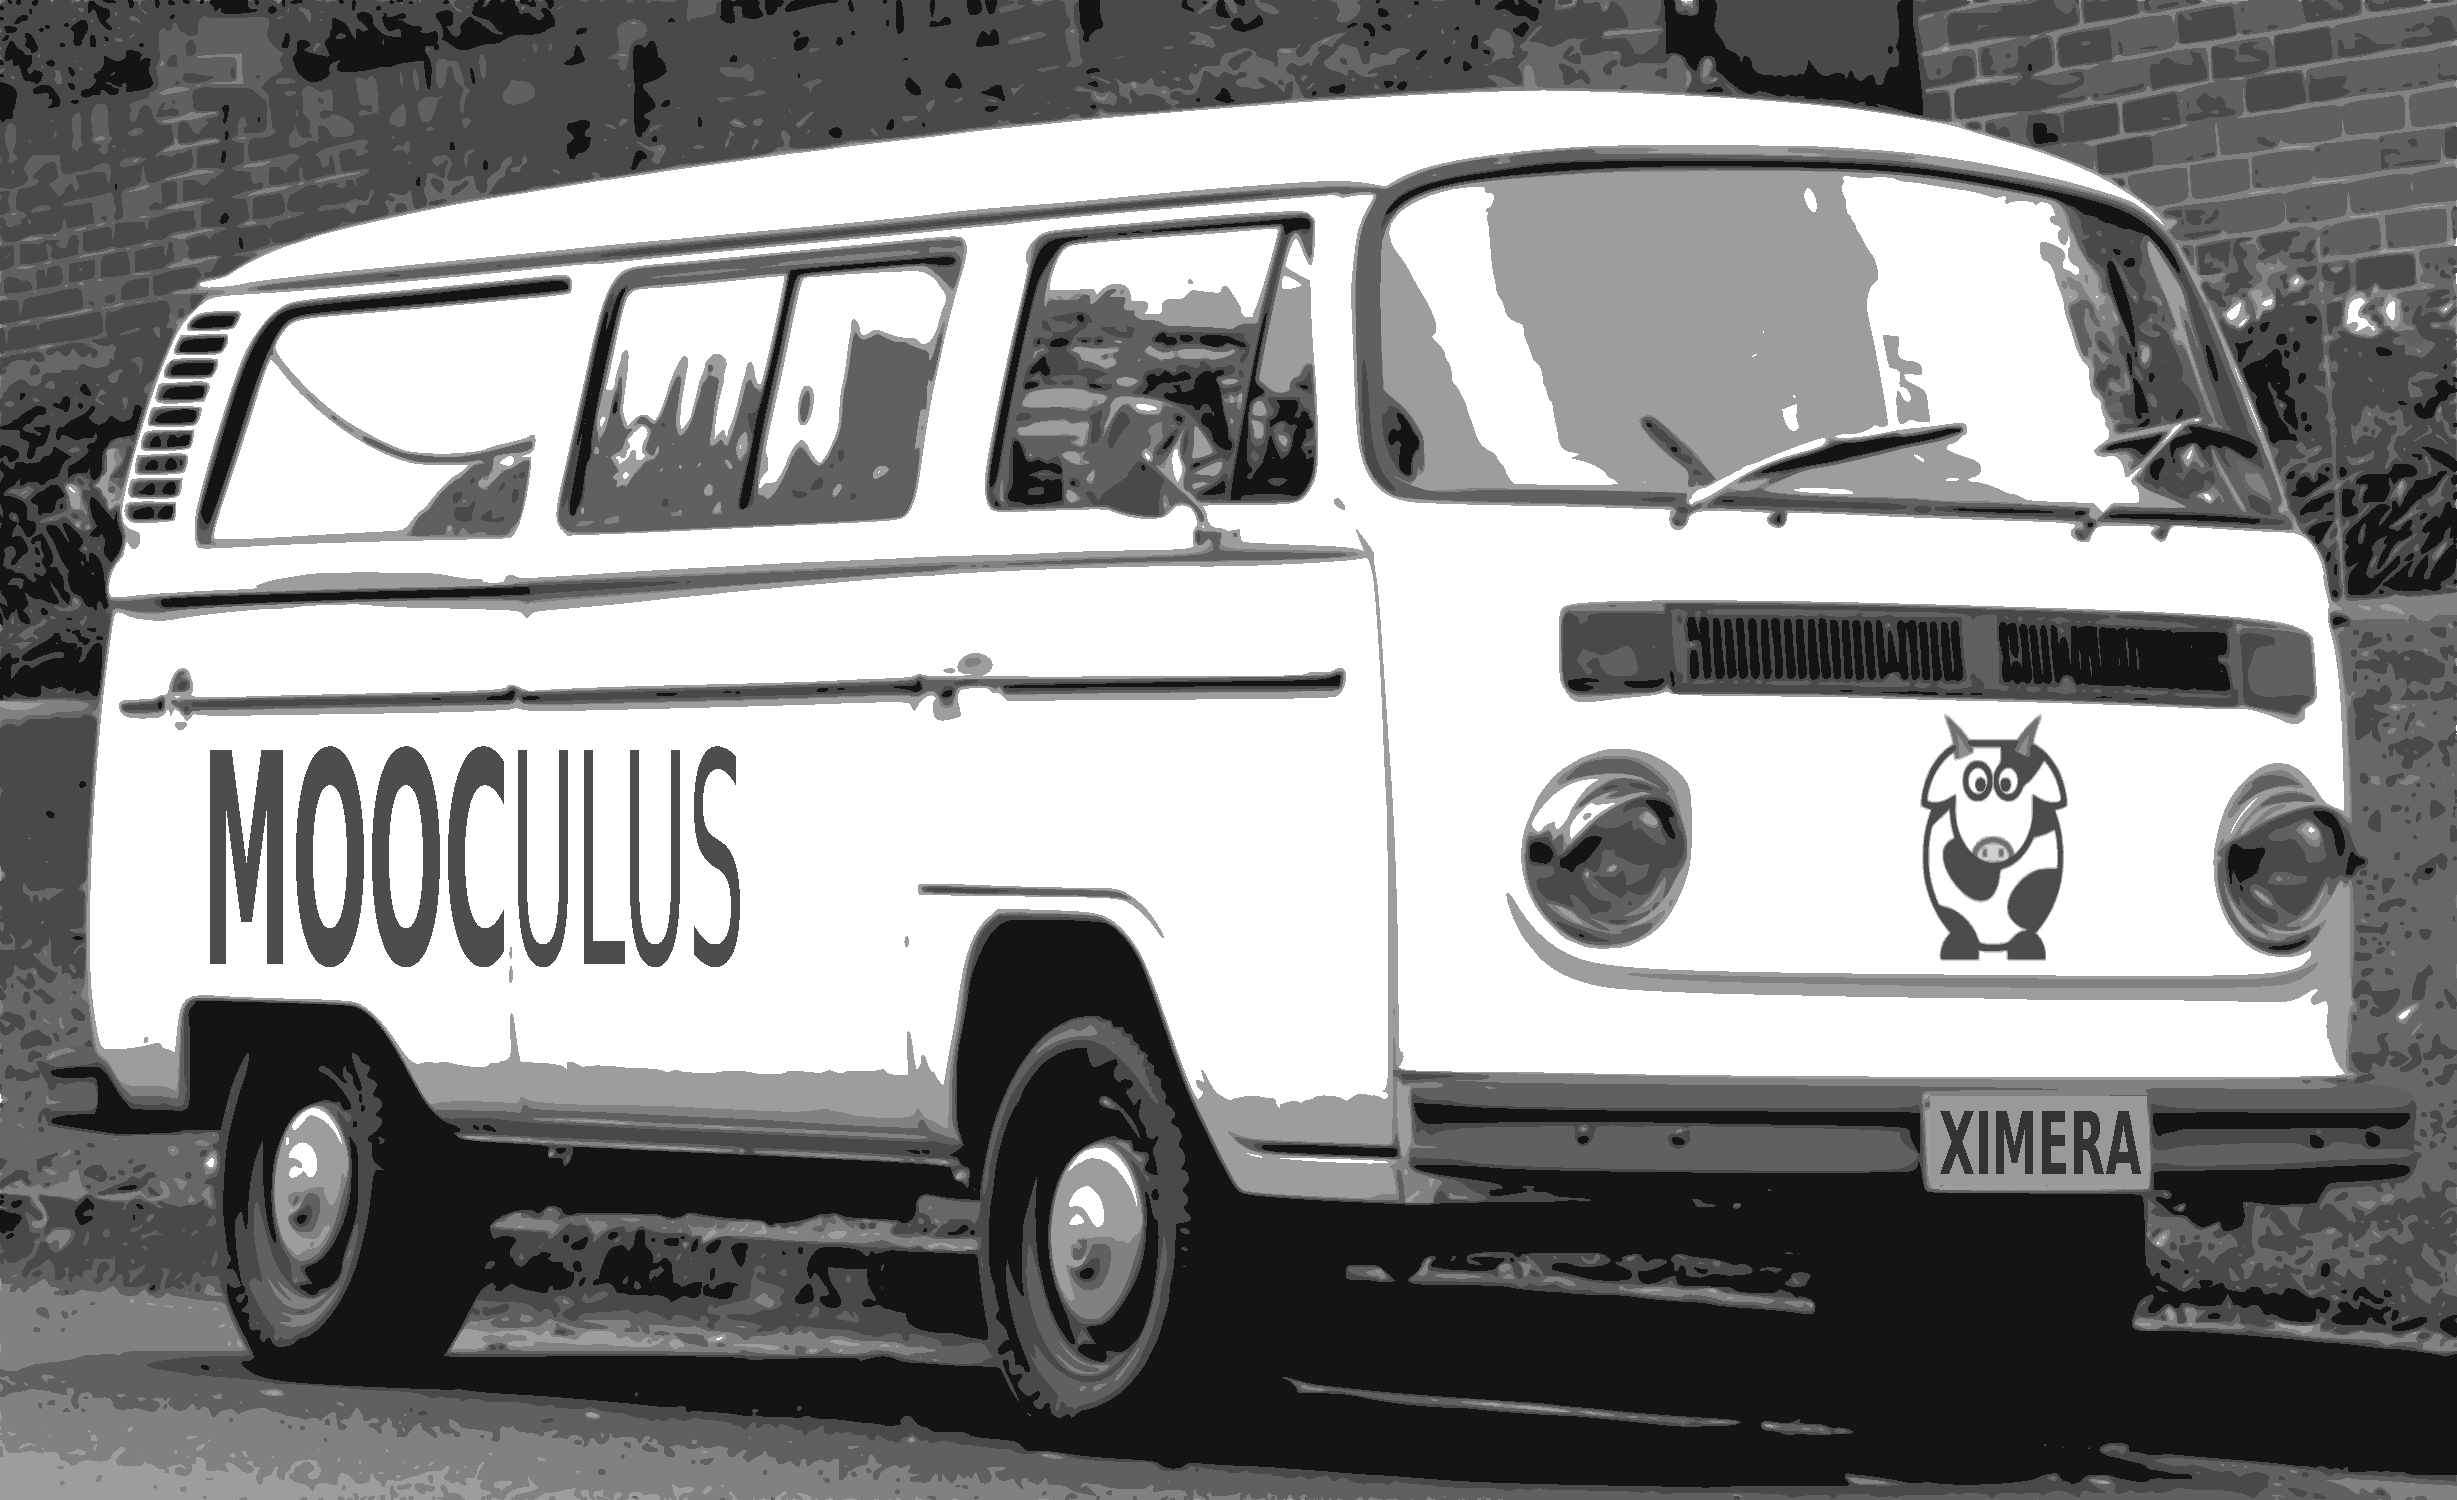
\includegraphics[width=3in]{mooculusMobile.pdf}
\end{image}
While the \textit{MOOCulus Mobile} might look pretty spiffy, it has
some problems, in particular, it has no speedometer!
Never-to-be-flustered, the MOOCulus team will just used their GPS to
help them compute the velocity. Let's see how. To do this, we need
some background. Urbana-Champaign is around 300 miles dead West of
Columbus. The position of the \textit{MOOCulus Mobile} is given by
\[
s(t) = 36t^2 -4.8t^3 \qquad\text{(miles from Columbus)}
\]
where $t$ is measured in hours. 

\begin{question}
Where is the MOOCulus Mobile at 0 hours? 
\end{question}


\begin{question}
Where is the MOOCulus Mobile at 5 hours? 
\end{question}

\begin{question}
What is the average velocity for the MOOCulus Mobile on the interval
$[0,5]$?
\end{question}

Now let's get a bit crazy, consider this interval:
\[
I_h = 
\begin{cases}
[2+h,2]  & \text{if $-1<h<0$}, \\ %% note this is MORE correct than std books
[2,2+h]  & \text{if $0<h<1$}. 
\end{cases}
\]

\begin{question}
What is this interval when $h = 0.5$?
\end{question}

\begin{question}
What is this interval when $h = -0.5$?
\end{question}

\begin{question}
Write a formula that will compute the average velocity of the
\textit{MOOCulus Mobile} for any given value of $h$.
\end{question}

This method described above may be fine for a robot that is computing
velocity from position using raw data. However, we are human beings
and not robots. What would really help us out is a formula. 



\begin{question}
Given a formula for position, how do we find a formula for velocity?
\end{question}

\begin{xarmaBoost}
Write down at least \textbf{five} questions for this lecture. After
you have your questions, label them as ``Level 1,'' ``Level 2,'' or ``Level 3'' where:
\begin{description}
\item[Level 1] Means you know the answer, or know exactly how to do
  this problem.
\item[Level 2] Means you think you know how to do the problem, or will
  soon learn how to do the problem.
\item[Level 3] Means you have no idea how to do the problem.
\end{description}
  \begin{freeResponse}
  \end{freeResponse}
\end{xarmaBoost}

\end{document}
